%!TEX root=paper/paper.tex
\section{Related Work}\label{sec:related_work}

Our work spans across several sub-fields of computer vision.
Here we cover the necessary background, ordered by applicability to each chapter of this thesis.

\subsection{Detection}

\PM{Features}
Classically, the best recent performance has come from detectors that use gradient-based features to represent objects as either a collection of local patches or as object-sized windows \parencite{Dalal2005,Lowe2004}.
Classifiers are then used to distinguish between featurizations of a given class and all other possible contents of an image window.
For state-of-the-art performance, the object-sized window models are augmented with parts \parencite{Felzenszwalb2010a}, and the bag-of-visual-words models employ non-linear classifiers \parencite{Vedaldi2009}.
In \autoref{sec:det_chapter}, we employ the widely used Deformable Part Model detector \parencite{Felzenszwalb2010a}.

\PM{CNNs}
Most recently, best performance is obtained not with hand-designed features but with those learned on large-scale labeled datasets such as ImageNet \parencite{Deng-CVPR-2009} by a deep convolutional neural network (CNN) such as AlexNet \parencite{Krizhevsky-NIPS-2012}.
This has prompted attempts to apply these computationally expensive methods to detection \parencite{Erhan-CVPR-2014,Sermanet-ICLR-2014}.
The \emph{R-CNN} method of \cite{Girshick-CVPR-2014} in particular is powerful but slow, requiring costly processing of many windows.
Recent work from \cite{He-ECCV-2014} (SPP-net) sustained the high performance of R-CNN while decreasing the running time by an order of magnitude.
Our work in \autoref{sec:ccnn_chapter} is evaluated in the R-CNN framework, but applies to the SPP-net method also.

\PM{Windows}
Window proposal is most often done exhaustively over the image space as a ``sliding window'', or inexhaustively with a bottom-up segmentation approach \parencite{Uijlings-IJCV-2013}.
Some approaches use ``jump windows'' (hypotheses voted on by local features) \parencite{Vedaldi2009,Vijayanarasimhan2011}, or a bounded search over the space of all possible windows \parencite{Lampert2008a}.
In all state-of-the-art systems, the window proposal step is conceptually separate from the feature extraction and classification.

\PM{Using feedback}
None of the best-performing systems treat window proposal and evaluation as a closed-loop system, with feedback from evaluation to proposal.
Some work has been done on this topic, mostly inspired by ideas from biological vision and attention research \parencite{Butko2009,Vogel2008}.
One application to the problem of visual detection picks features with maximum value of information in a Hough-voting framework \parencite{Vijayanarasimhan2010}.
Another uses nearest-neighbor lookups of image windows to sum offset vectors onto objects \parencite{Alexe2012a}.

\PM{Multi-class context}
Most detection methods train individual models for each class.
Work on inherently multi-class detection focuses largely on making detection time sublinear in the number of classes through sharing features \parencite{Torralba2007,Fan2005}.
Inter-object context has also been shown to improve detection \parencite{Torralba2004}.
A post-processing extension to detection systems uses structured prediction to incorporate multi-class context as a principled replacement for non-maximum suppression \parencite{Desai2009}.
In a standard evaluation setup, inter-object context plays a role only in post-filtering, once all detectors have been run.
In contrast, our work leverages inter-object context in the action-planning loop.

\PM{Scene context}
The most common source of context for detection is the \emph{scene} or other non-detector cues; the most common scene-level feature is the GIST \parencite{Oliva-IJCV-2001} of the image.
We use this source of scene context in our evaluation.
A critical summary of the main approaches to using context for object and scene recognition is given in \parencite{Galleguillos2010}.
For the commonly used PASCAL VOC dataset \parencite{pascal-voc-2010}, GIST and other sources of context are quantitatively explored in~\parencite{Divvala2009}.

\subsection{Classification}

\PM{Features}
%!TEX root=paper/paper.tex
\begin{figure}[ht]
\centering
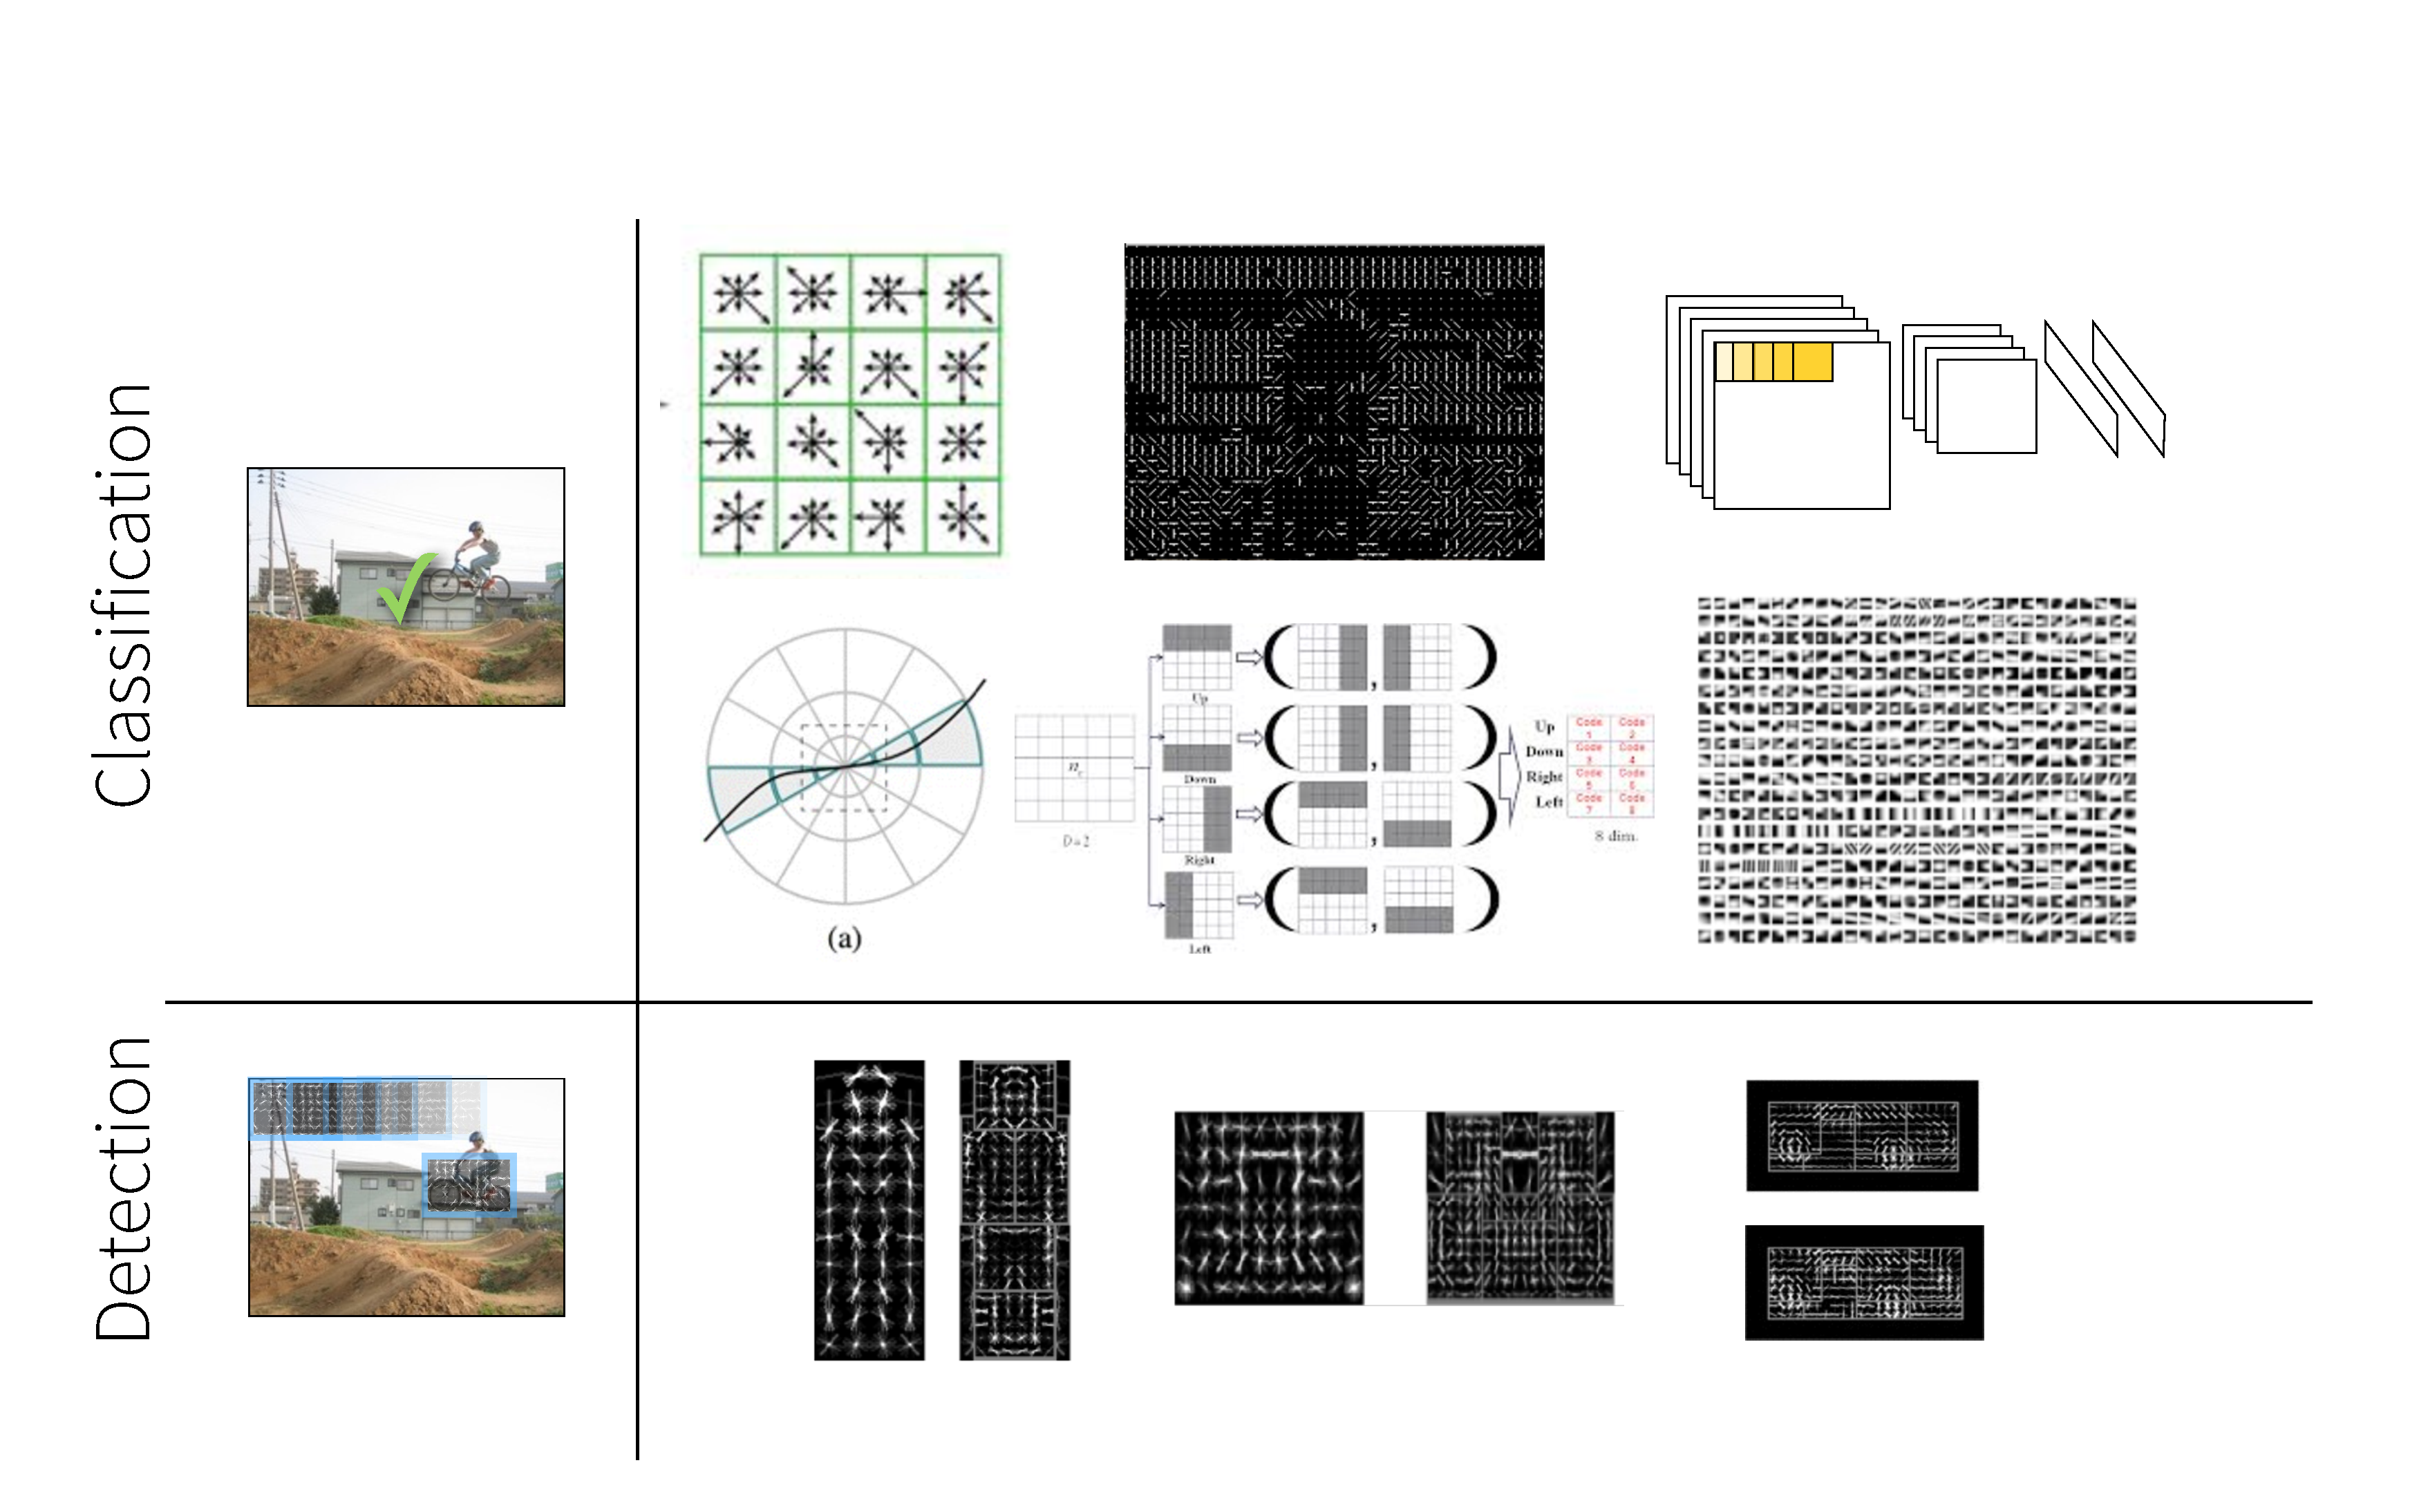
\includegraphics[width=\linewidth]{../../figures/features.pdf}
\caption[Summary of the variety of features for object detection and classification.]{
Summary of the variety of features for object detection and classification.
In reading order for classification: SIFT \parencite{Lowe2004}, HOG \parencite{Dalal2005}, CNN \parencite{Krizhevsky-NIPS-2012}, Self-Similarity \parencite{Shechtman2007}, Haar basis functions \parencite{Viola-IJCV-2004}, basis functions learned with sparse coding \parencite{Olshausen1996}.
In reading order for detection: person, bicycle, and car templates for the Deformable Part Model \parencite{Felzenszwalb2010a}.
}\label{fig:features}
\end{figure}


\PM{Visual features}
The field of computer vision has built up a small arsenal of features extracted from whole images or fixed-size patches.
These features differ in computational cost and target different sources of data -- for instance, the Haar wavelets feature of \cite{Viola-IJCV-2004} was designed for sequential appication in face recognition datasets, while the HOG feature of \cite{Dalal2005} was designed for template matching in pedestrian-detection datasets.
\autoref{fig:features} presents a sampling of the most used ones.
Recently, middle layers of CNN's trained on large image categorization datasets have provided a generally applicable feature that obtains top performance on a multitude of datasets \parencite{Donahue2013a}.

\PM{Feature selection}
The simplest way to limit the number of features used at test time is to $L_1$-regularize.
This method does not explicitly consider feature cost, nor is it able to evaluate features one by one, or to give an answer before all features are computed.
In Figures \ref{fig:model_cascade}, \ref{fig:model_mddag}, \ref{fig:model_tree}, \ref{fig:model_dag} and in the paragraphs below we explain more advanced methods, all of them treating feature selection as a sequential process.

\PM{Cascaded methods}
A well-known method to evaluate features sequentially is the cascaded boosted classifier of \cite{Viola-IJCV-2004} (updated by \cite{Bourdev-CVPR-2005} with a soft threshold), which is able to quit evaluating an instance before all features are computed---but feature cost was not considered.
The cost-sensitive cascade of \cite{Chen-AISTATS-2012} optimizes stage order and thresholds to jointly minimize classification error and feature computation cost.
\autoref{fig:model_cascade} represents this model.
\cite{Xu-ICML-2012} and \cite{Grubb-AISTATS-2012} separately develop a variant of gradient boosting for training cost-sensitive classifiers; the latter prove near-optimality of their greedy algorithm with submodularity results.
Their methods are tightly coupled to the stage-wise regression algorithm.
Cascades are not dynamic policies: they cannot change the order of execution based on observations obtained during execution, which is our goal.

\PM{Dynamic methods}
In contrast, \emph{Label trees} guide an instance through a tree of classifiers; their structure is determined by the confusion matrix or learned jointly with weights \parencite{Deng-NIPS-2011}.
\cite{Xu-ICML-2013} learn a cost-sensitive binary tree of weak learners using an approach similar to the cyclic optimization of \parencite{Chen-AISTATS-2012}.
The state space of such tree methods is visualized in \autoref{fig:model_tree}.
A fully general DAG -- instead of a tree  -- over the state space is proposed by \cite{Gao-NIPS-2011} under the name of \emph{active classification}, and visualized in \autoref{fig:model_dag}.
Their method myopically selects the next feature based on expected information gain given the values of the already selected features.
Since it is based on locally weighted regression, \emph{active classification} is highly costly at test time.
\cite{Ji-PR-2007} also formulate cost-sensitive feature selection generatively, as an HMM conditioned on actions, but select actions myopically, again at signficant test time cost.

\PM{Reinforcement Learning}
Just like active classification, our method and the three methods below can learn any possible policy.
\cite{DulacArnold-ML-2012} present an MDP-based solution to ``datum-wise classification'', with an action space comprised of all features and labels, recently extended to region-based processing \parencite{DulacArnold-ICLR-2014}.
This independently-conducted work is closely related to ours, with differences in defining the action space and learning mechanism.
\cite{HeHe-ICMLW-2012} formulate an MDP with features and a single classification step as actions, but solve it via imitation learning of a greedy policy.
\cite{Trapeznikov-ML-2012} provides another variation on this formulation.
Another notable work is the method of \cite{Benbouzid-ICML-2012}, graphically presented in \autoref{fig:model_mddag}, which formulates an MDP that simply extends the traditional sequential boosted classifier with an additional \emph{skip} action, significantly limiting the space of learnable policies.
This ``MD-DAG'' method is able to learn only a subset of all possible policies.

\PM{Misc}
Less directly related -- but exciting for its novelty -- is the work of \parencite{Weiss-ICCV-2013}, who apply simple introspection to structured models for a significant speedup of human pose estimation.
Another exciting direction is theoretical analysis based on adaptive submodularity \parencite{Golovin-and-Krause-2010-JAIR}.
In vision, there is an application of such results to detection with humans in the loop \parencite{Chen-2014-ICML}.
In robotics, an adaptively submodular objective was successfully formulated for the problem of grasping \parencite{Javdani2012}.

%!TEX root=paper/thesis.tex
\begin{figure}[h!]
\centering
\begin{subfigure}[t]{0.48\linewidth}
    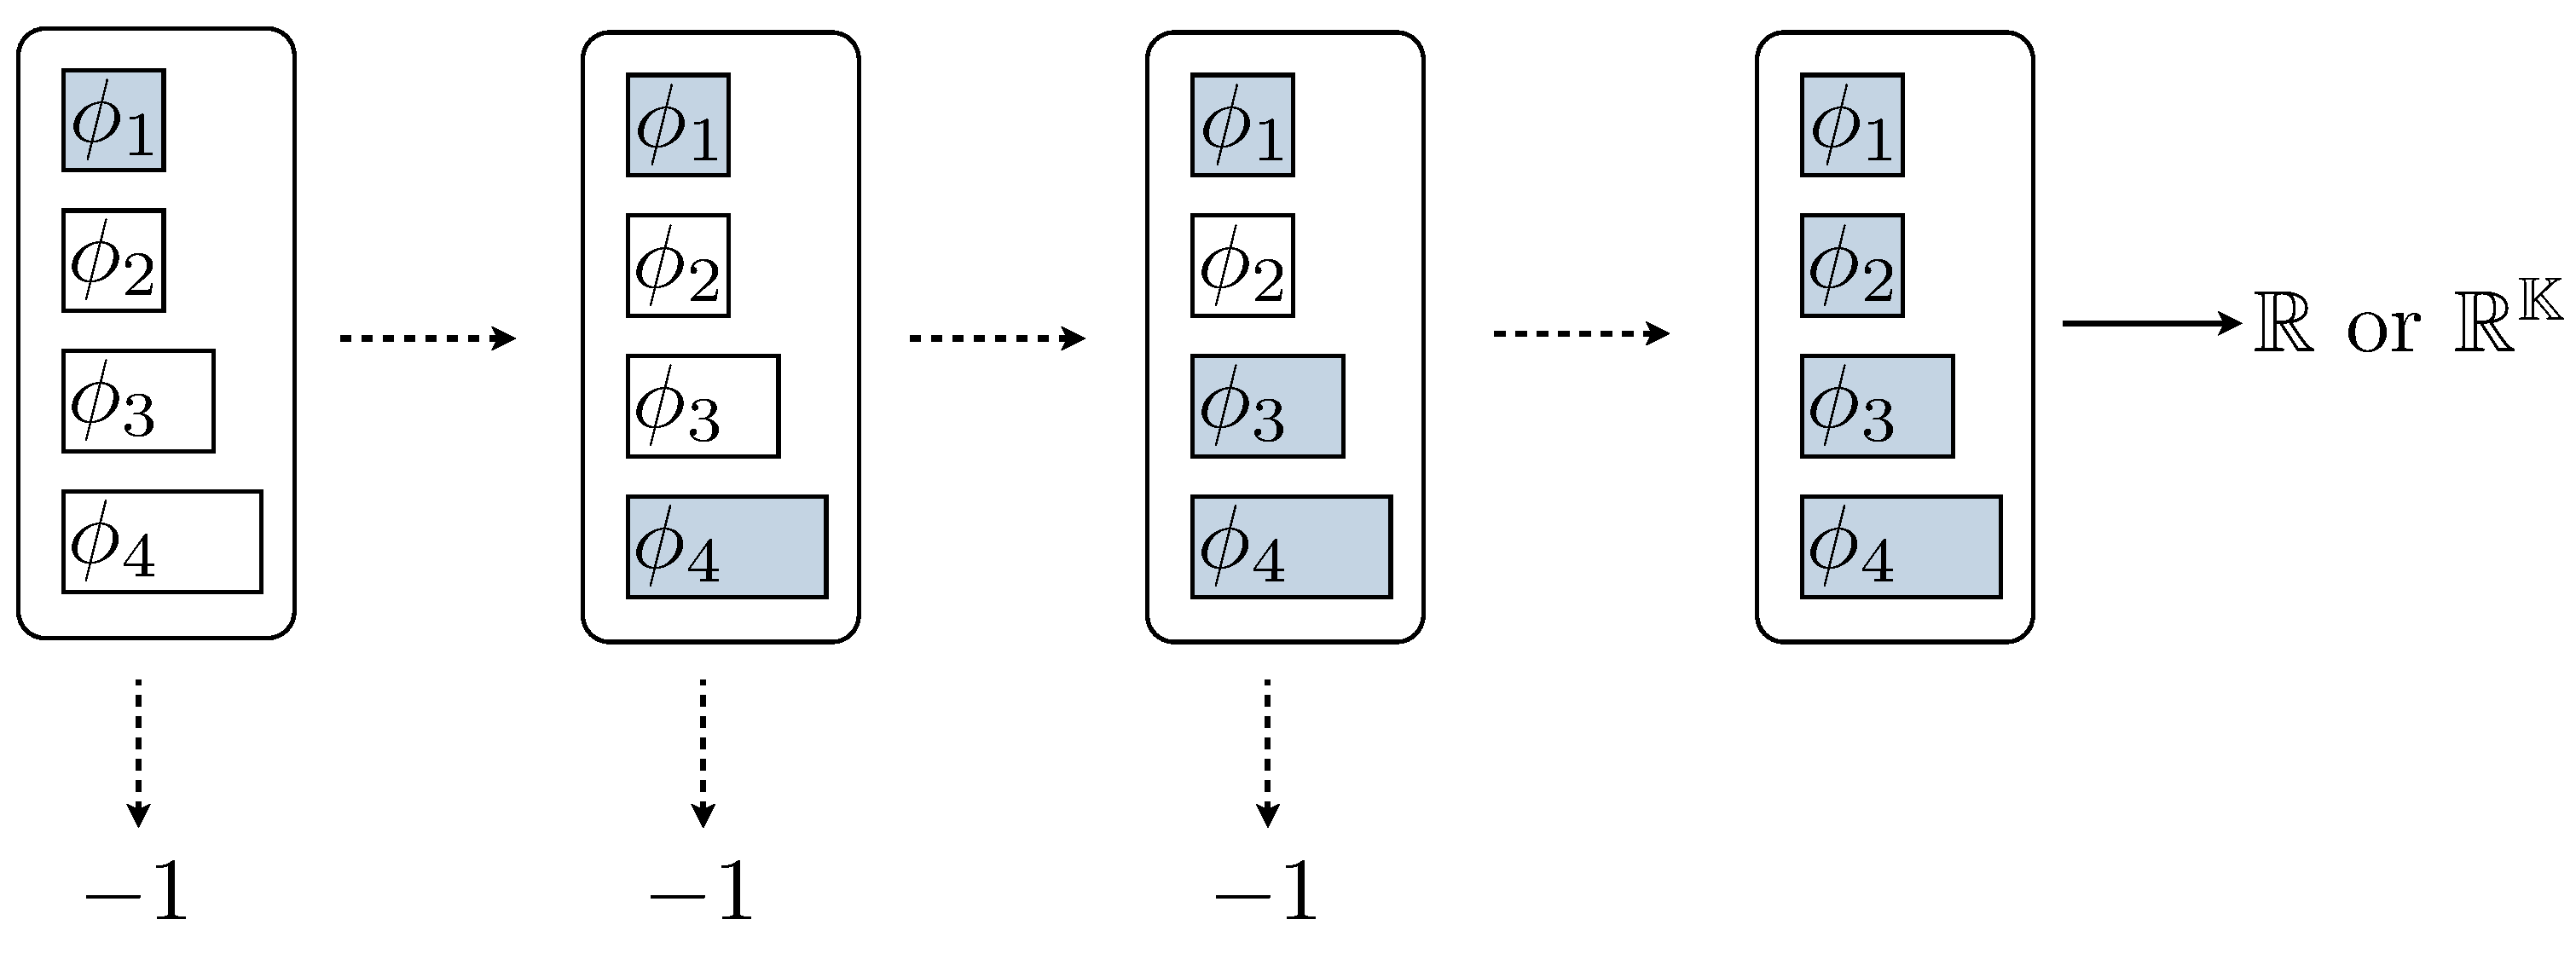
\includegraphics[width=\linewidth]{../../figures/models/cascade}
    \caption{
\textbf{Cascade}
In addition to the feature computation actions, the classifier is augmented with a rejection action.
The cascade is Anytime in a limited way, as only the rejection answer can be given before all features are evaluated.
Furthermore, the fixed order of the cascade is not robust to the fact that different images benefit from different features.
}
\end{subfigure}\hfill%
\begin{subfigure}[t]{0.48\linewidth}
    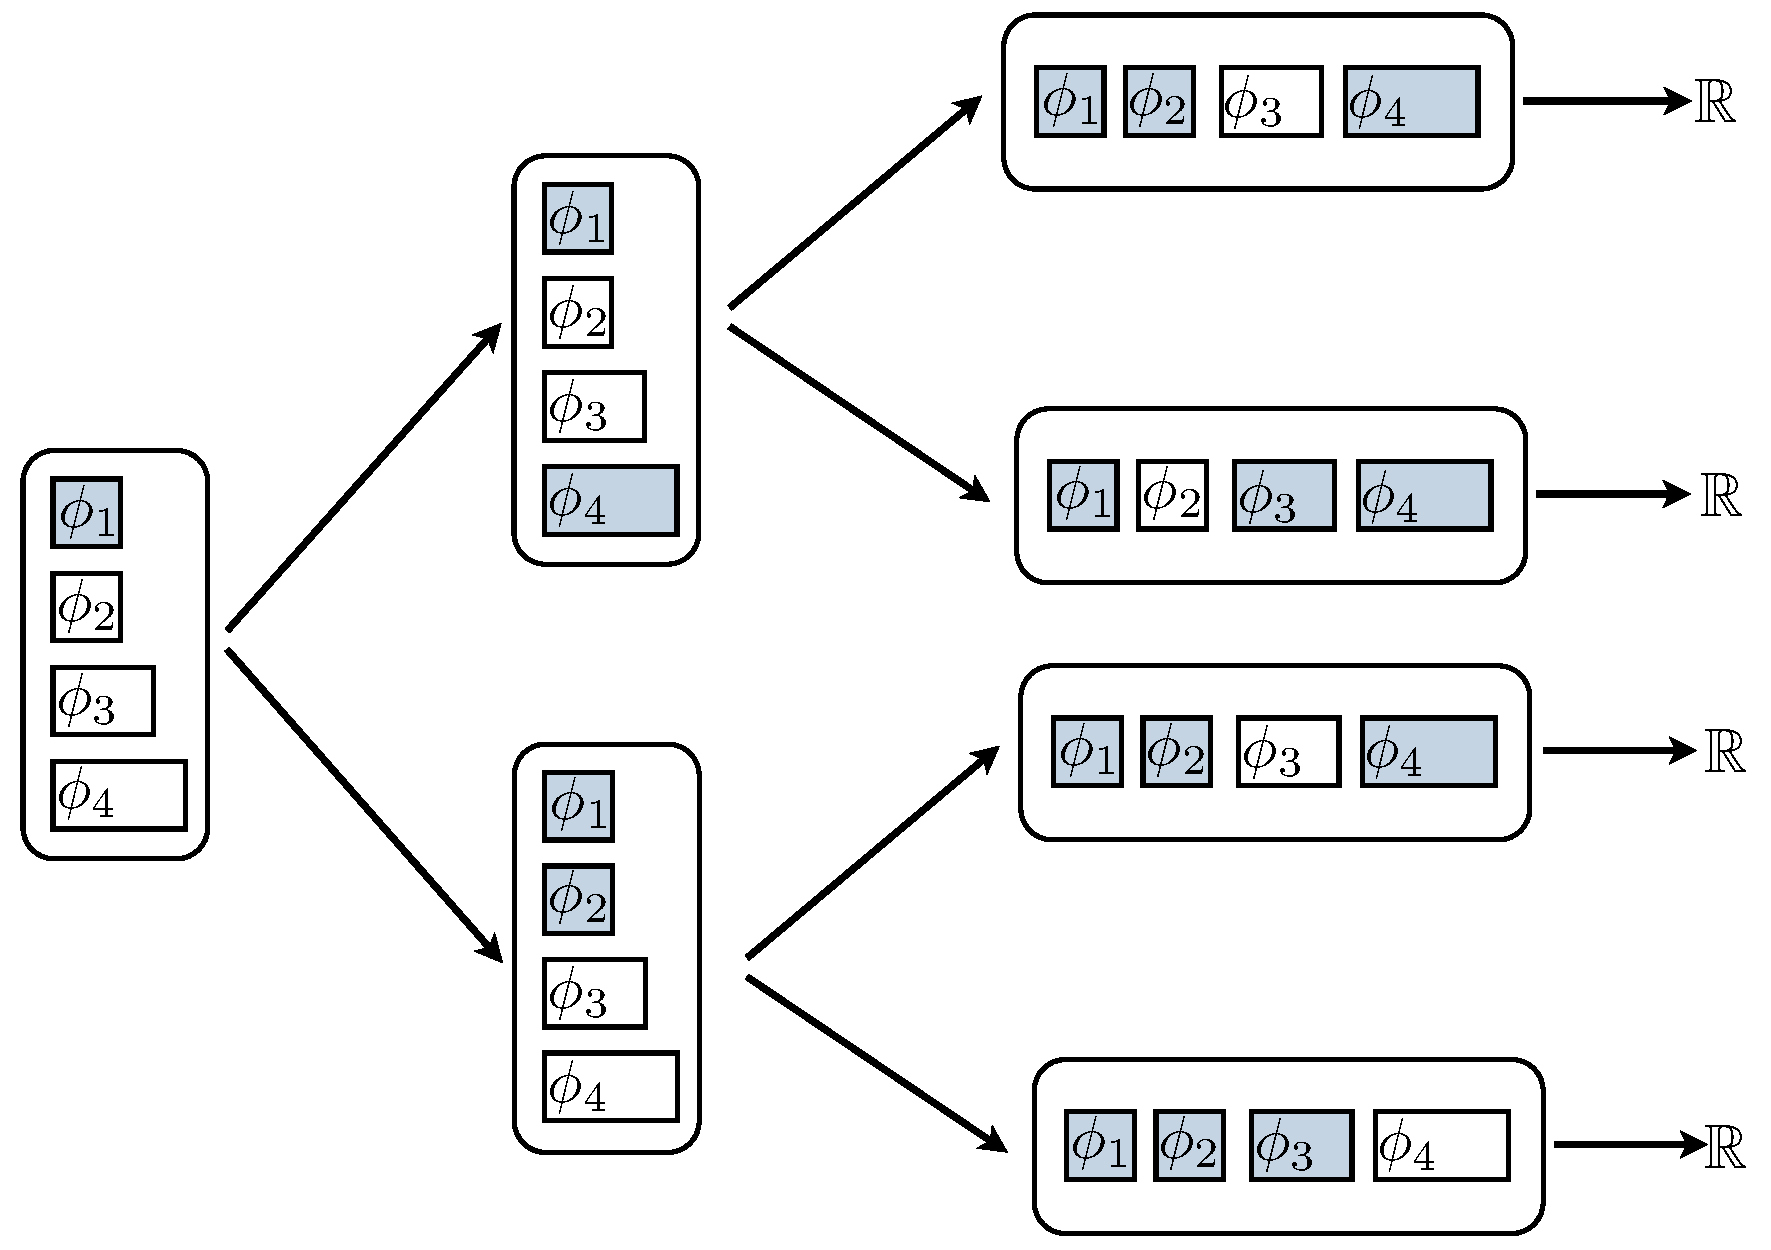
\includegraphics[width=\linewidth]{../../figures/models/tree}
    \caption{
Methods such as \cite{Xu-ICML-2012} find a tree-structured policy for computing features.
Classification answers are given only at the leaf nodes.
    }
\end{subfigure}\\
\begin{subfigure}[t]{0.48\linewidth}
    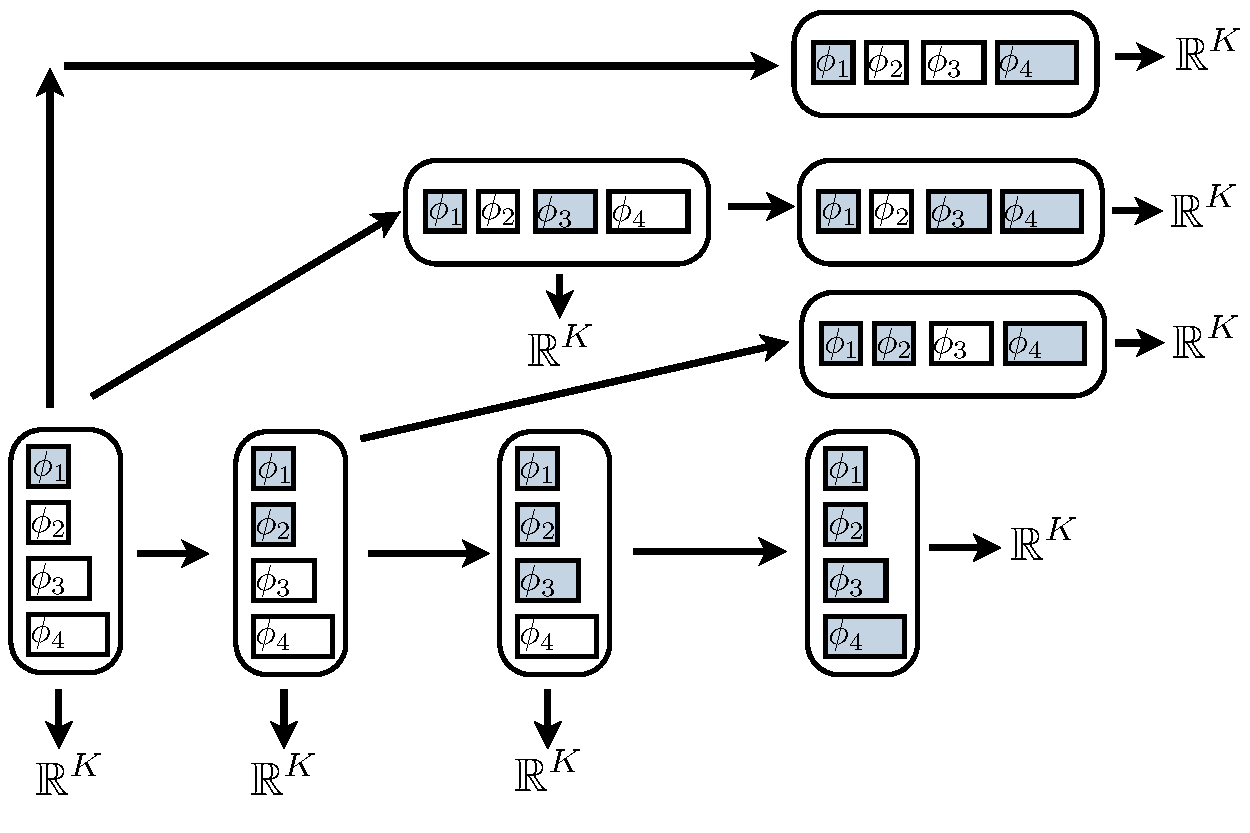
\includegraphics[width=\linewidth]{../../figures/models/benbouzid}
    \caption{
The method of \cite{Benbouzid-ICML-2012} augments the traditional cascade with an additional Skip action, which allows learning a more robust policy.
}
\end{subfigure}\hfill%
\begin{subfigure}[t]{0.48\linewidth}
    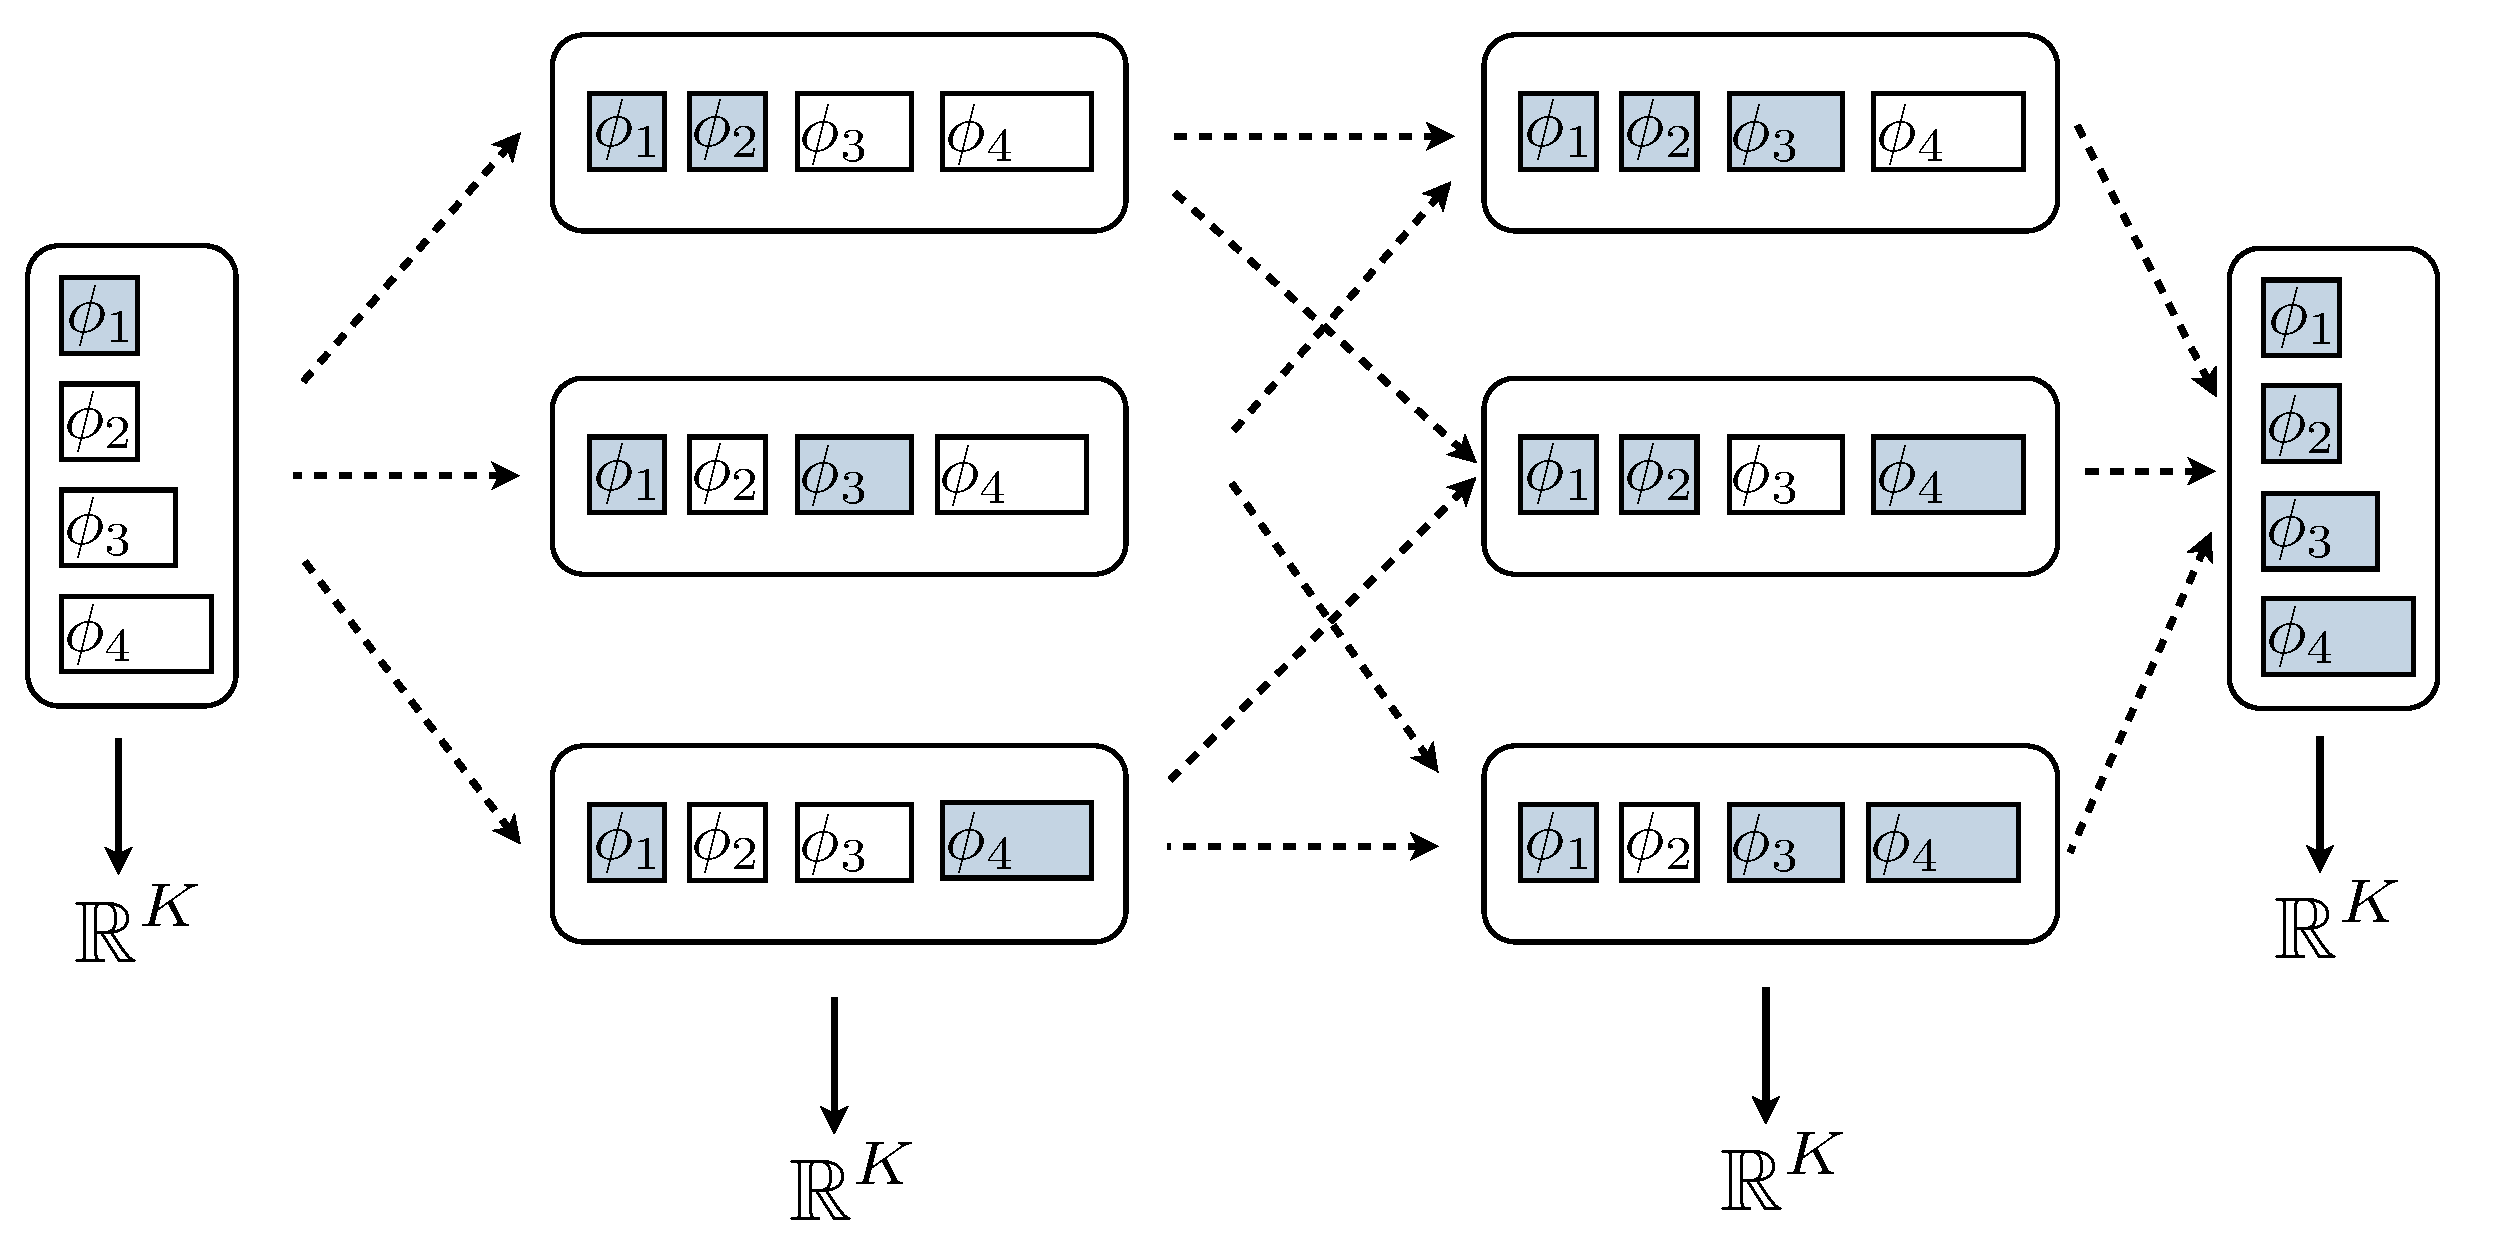
\includegraphics[width=\linewidth]{../../figures/models/dag}
    \caption{
In this work and in methods such as \cite{Gao-NIPS-2011}, the policy is a DAG over selected-feature subsets, which allows actions to be taken in an entirely flexible order.
We are also able to give the classification answer from all states, making our work truly Anytime.
    }
\end{subfigure}
\caption{
Different models for classification with sequential feature selection.
}\label{fig:models}
\end{figure}


\subsubsection{Feature Combination}

\PM{Multiple Kernel Learning}
For SVM-based classifiers, \emph{Multiple Kernel Learning} (MKL) provides a way to train classifiers using an automatically weighted combination of kernels \parencite{Lanckriet2004}.
It has been shown that MKL is outperformed by boosting single-kernel classifiers \parencite{Gehler2009}.
Of course, if all classifiers are linear, then combining outputs of classifiers trained on different feature channel with another classifier is equivalent to training one classifier on all features at once.

\PM{Value imputation}
The imputation problem is faced in the \emph{collaborative filtering} literature, working on problems such as the Netflix Prize \parencite{Koren-2009}.
Matrix factorization methods, commonly based on the Singular Value Decomposition (SVD), are often employed.
Our problem is significantly different in that at training time, all values are fully observed --- and the final task is classification, not simple imputation.
Imputation approaches have also been explored in genomics work, where the real-world data is often missing a large portion of the observations \parencite{Hastie-1999}.

\section{Style Recognition}

Most research in computer vision addresses recognition and reconstruction, independent of image style.
A few previous works have focused directly on image composition, particularly on the high-level attributes of beauty, interestingness, and memorability.

\PM{Aesthetic Rating}
Most commonly, several previous authors have described methods to predict aesthetic quality of photographs.
Datta et al.~\parencite{Datta-ECCV-2006}, designed visual features to represent concepts such as colorfulness, saturation, rule-of-thirds, and depth-of-field, and evaluated aesthetic rating predictions on photographs; The same approach was further applied to a small set of Impressionist paintings~\parencite{Li-SP-2009}.
The feature space was expanded with more high-level descriptive features such as ``presence of animals'' and ``opposing colors'' by Dhar et al., who also attempted to predict Flickr's proprietary ``interestingness'' measure, which is determined by social activity on the website~\parencite{Dhar-CVPR-2011}.
Gygli et al.~\parencite{Gygli-ICCV-2013} gathered and predicted human evaluation of image interestingness, building on work by Isola et al.~\parencite{Isola-CVPR-2011}, who used various high-level features to predict human judgements of image memorability.
In a similar task, Borth et al.~\parencite{Borth-MM-2013} performed sentiment analysis on images using object classifiers trained on adjective-noun pairs.

\PM{AVA and Attributes}
Murray et al.~\parencite{Murray-CVPR-2012} introduced the Aesthetic Visual Analysis (AVA) dataset, annotated with ratings by users of DPChallenge, a photographic skill competition website.
The AVA dataset contains some photographic style labels (e.g., ``Duotones,'' ``HDR''), derived from the titles and descriptions of the photographic challenges to which photos were submitted.
Using images from this dataset, Marchesotti and Peronnin~\parencite{Marchesotti-BMVC-2013} gathered bi-grams from user comments on the website, and used a simple sparse feature selection method to find ones predictive of aesthetic rating.
The attributes they found to be informative (e.g., ``lovely photo,'' ``nice detail'') are not specific to image style.

\PM{Visual Art}
Features based on image statistics have been successfully employed to detect artistic forgeries \parencite{Lyu-PNAS-2004}.
Such work focuses on extremely fine-scale discrimination between two very similar classes, and has not been applied to broader style classification.
Several previous authors have developed systems to classify classic painting styles, including \parencite{keren2002,shamir2010}.
These works consider only a handful of styles (less than ten apiece), with styles that are visually very distinct, e.g., Pollock vs.~Dal\'{\i}.
These datasets comprise less than 60 images per style, for both testing and training.
\cite{Mensink2014} provide a larger dataset of artworks, but do not consider style classification as its own problem.

\PM{Style vs. Content}
Separate from the application domain of vision, some machine learning research has attempted to separate style from content \parencite{Tenenbaum2000}.
In particular, Neural Network researchers have provided interesting recent results: \cite{Taylor-ICML-2009} use a Restricted Boltzmann Machine to separately consider style and content for the problem of human gait recognition, and \cite{Graves-arxiv-2013} uses a Long Short-Term Memory recurrent neural network to generate realistic handwriting in a multitude of styles.
